%! alt Circle omega with centre O and triangle ABC inscribed, A at the top. Chord XY is horizontal and passes through P on AB and Q on AC, with XP = 64, PQ = 56 and QY = 48. The tangent at A is parallel to XY, and the radius OA meets XY at right angles at its midpoint M.
%! after_paragraph 2
%! scale 1/27
% The shared preamble of every Kyuclid figure. pipeline/figures turns these colours into theme-aware paint,
% and refuses any other colour, so draw only with them:
%   figink (lines and labels), figaux (construction lines), figaccent (the object the argument turns on),
%   figtint and figaccenttint (light fills).
\documentclass[border=1.5pt]{standalone}
\usepackage{tkz-euclide}
\definecolor{figink}{RGB}{0,0,0}
\definecolor{figaux}{RGB}{85,85,85}
\definecolor{figaccent}{RGB}{192,57,43}
\definecolor{figtint}{RGB}{221,221,221}
\definecolor{figaccenttint}{RGB}{245,213,208}
% tkz-euclide's defaults draw circles, compasses and marks in 50% grey and fill points with a tint.
\makeatletter
\def\tkz@otherlinecolor{figink}
\def\tkz@euc@circlecolor{figink}
\def\tkz@euc@compasscolor{figink}
\def\tkz@euc@mkcolor{figink}
\def\tkz@mk@fill{figink}
\def\tkz@euc@pointfillcolor{figink}
\makeatother
\tkzSetUpLine[color=figink,line width=.7pt]
\tkzSetUpArc[color=figink,line width=.7pt]
\tkzSetUpCompass[color=figink,line width=.5pt]
\tkzSetUpPoint[color=figink,fill=figink,size=3.1pt]
\tikzset{
  every picture/.style={line cap=round,line join=round,color=figink},
  circle style/.append style={color=figink,line width=.7pt},
  aux/.style={color=figaux,line width=.45pt,dash pattern=on 2.6pt off 2pt},
  key/.style={color=figaccent,line width=1pt},
  mk/.style={color=figink,line width=.5pt},
  lbl/.style={color=figink,inner sep=2.2pt},
  len/.style={color=figink,inner sep=1.5pt,font=\small},
}

\begin{document}
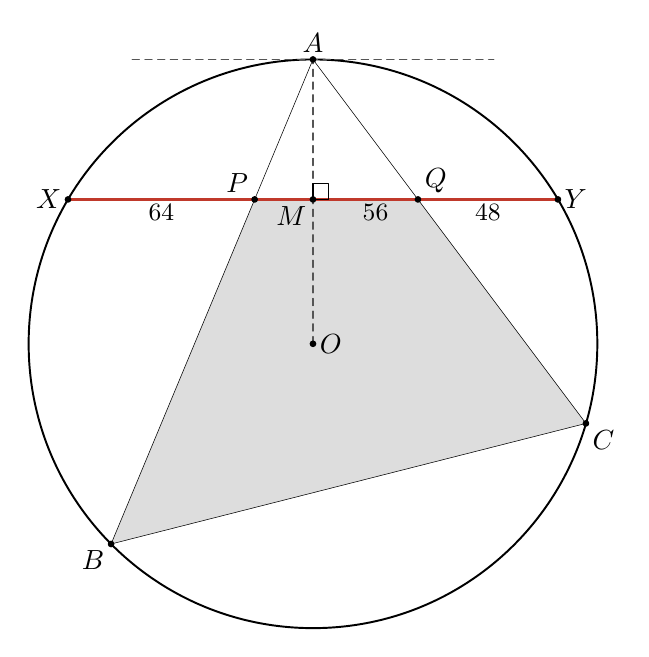
\begin{tikzpicture}
\tkzDefPoint(0.0,0.0){O} %! O = (0, 0)
\tkzDefPoint(0.0,3.6111111){A} %! A = (0, 195/2)
\tkzDefPoint(0.0,1.8333333){M} %! M = (0, 99/2)
\tkzDefPoint(-3.1111111,1.8333333){X} %! X = (-84, 99/2)
\tkzDefPoint(3.1111111,1.8333333){Y} %! Y = (84, 99/2)
\tkzDefPoint(-0.74074074,1.8333333){P} %! P = (-20, 99/2)
\tkzDefPoint(1.3333333,1.8333333){Q} %! Q = (36, 99/2)
\tkzDefPoint(-2.5641026,-2.5427350){B} %! B = lerp(A, P, 180/52)
\tkzDefPoint(3.4666667,-1.0111111){C} %! C = lerp(A, Q, 156/60)
\tkzDefPoint(-2.2962963,3.6111111){T} %! T = (-62, 195/2)
\tkzDefPoint(2.2962963,3.6111111){U} %! U = (62, 195/2)
%! fact on_circle(A, O, 195/2)
%! fact on_circle(B, O, 195/2)
%! fact on_circle(C, O, 195/2)
%! fact on_circle(X, O, 195/2)
%! fact on_circle(Y, O, 195/2)
%! fact concyclic(B, C, Q, P)
%! fact dist(X, P) == 64
%! fact dist(P, Q) == 56
%! fact dist(Q, Y) == 48
%! fact perp(O, A, X, Y)
%! fact midpoint(M, X, Y)
%! fact tangent(O, 195/2, T, U)
%! fact parallel(T, U, X, Y)
%! fact dist(A, B) == 180
%! fact dist(A, C) == 156
%! fact dist(B, C) == 168
\tkzFillPolygon[color=figtint](B,P,Q,C)
\tkzDrawCircle(O,A)
\tkzDrawSegment[aux](T,U)
\tkzDrawSegment[aux](O,A)
\tkzDrawPolygon(A,B,C)
\tkzDrawSegment[key](X,Y)
\tkzMarkRightAngle[size=.2,mk](A,M,Y)
\tkzDrawPoints(O,A,B,C,X,Y,P,Q,M)
\tkzLabelPoint[above,lbl](A){$A$}
\tkzLabelPoint[below left,lbl](B){$B$}
\tkzLabelPoint[below right,lbl](C){$C$}
\tkzLabelPoint[left,lbl](X){$X$}
\tkzLabelPoint[right,lbl](Y){$Y$}
\tkzLabelPoint[above left,lbl](P){$P$}
\tkzLabelPoint[above right,lbl](Q){$Q$}
\tkzLabelPoint[below left,lbl](M){$M$}
\tkzLabelPoint[right,lbl](O){$O$}
\tkzLabelSegment[below,len](X,P){$64$}
\tkzLabelSegment[below,pos=.74,len](P,Q){$56$}
\tkzLabelSegment[below,len](Q,Y){$48$}
\end{tikzpicture}
\end{document}
